\clearpage
\begin{flushright}
	\textit{Лекция №2}
	\textit{2015.09.08}
\end{flushright}

Каналы это специальные процессоры. Процессор может переключиться на другую работу, пока канал работает с внешним устройством. Когда канал заканчивает работу – вызывается аппаратное прерывание. 

Русские ЭВМ: БЭСМ большая электронная счетная машина. БЭСМ 6 – 1милл вычислений в сек. Архитектура основа на принципе распараллеливания. Всё своё. В это время в Америке интенсивное развитие. Решили перейти на единую серию и все силы брошены на копирование американцев. В результате созданы свои схемы, запущено производство интегральных схем, выход годных хуже в 100 раз.

\begin{figure}[H]
  \centering
  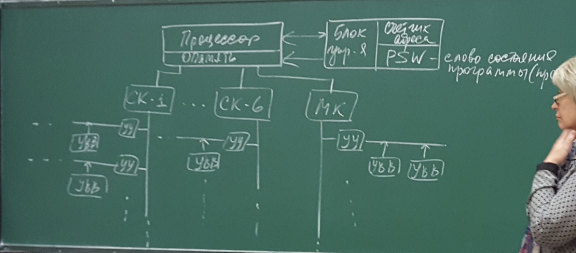
\includegraphics[width=\textwidth]{pic/1.png}
  \caption{Архитектура ЕС ЭВМ}
  \label{pic:es_evm}
\end{figure}

\ref{pic:es_evm} Отражает канальную архитектуру, передирали c ибм360 – первая линейка вычислительных машин.

Два вида каналов:
\begin{enumerate}
\item селекторный – в каждый момент времени каждый канал работает с единственным устройством ввода – вывода. Работают с быстрыми устройствами.;
\item мультиплексорный - может работать с несколькими устройства ввода вывода. Работают с медленными устройствами.
\end{enumerate}

Чтобы ускорить переключение с одного задания на другое стали загружать в оперативку большое число программ. Чтобы иметь возможность управлять набором программ был создан язык управления заданиями. В результате любая программа предварялась командами на языке управления заданиями. Указывался транслятор, максимальный необходимый объем ОЗУ и время выполнения программы. На основе этих данных система решала порядок выполнения программ в рабочей смеси. Это пакетный режим. С элементной базой и с архитектурой развивались внешние устройства.  

Появились электронно-лучевых мониторы. Были на запоминающих трубках. Появились терминалы. Теперь ЦП должна обеспечивать человеку комфортную среду работы (не должен ждать неопределенное время).  Система должная обеспечить гарантированное время. Называли это - системы разделения времени путем квантования процессорного времени. Каждой программе выделяется фиксированный квант процессора.

\section{4 поколение. 1970 – н.в.}

Большие и Сверх Большие интегральные схемы. 

Сеймур Крей создал первый суперкомпьютер Крей 1 с первым конвейером.
Создание intel 8080. Затем 16 разрядный процессор + 20 разрядная шина адреса intel 8088. Поставлена MS-DOS.

Для PDP написана Unix – система разделения времени. К PDP можно подключать большое количество терминалов. Для ускорения написания работы между операционной системой и шеллом разработчики написали СИ для нужд системного программирования. ОС Малтикс – система разделения времени для обучения. 
PDP 11 поставлена в научные центры Америки с открытым кодом ядра.
Мультипрограммные системы пакетной обработки – в памяти большое кол-во программ. 

МС-ДОС для компов intel 8088. Однопрограммная ось. Поддерживала перемещаемые сегменты. 

Для ибм370 написана VM (операционная система). Позволяла как задачи запускать операционные системы пакетной обработки, разделения времени, реального времени. Одновременно выполнялись несколько операционных систем. Пользователь заказывал ось, какую он хотел. 

\subsubsection{Реальное время} речь идет о ПО. Реальное время по отношению к осям имеет специфический смысл. Любое устройство работает в реальном времени. Операционные системы реального времени предназначены для управления процессами реального времени. Это процессы, которые обслуживают внешние по отношению к системе устройства. Они называются системами РВ потому что должны обеспечивать определенные временные характеристики работы этих процессов, которые определяются характеристиками внешними устройствами. Никогда про РВ не говорят быстрые или медленные процессы, это чушь. Система должна обрабатывать полученную информацию за время меньшее чем период опроса датчиков. Т.е. управляющее воздействие системы должно быть сформировано за время, определенное характеристиками конкретной подсистемы летательного аппарата. Это РВ. Самолет и его системы работают в реальном времени.

Видео и аудио. Телевизионное изображение – изображение с регенерацией. Для человека характерно инерционность зрения. Глаз сохраняет картинку на 1/24 секунду. Частота смены кадров в телевизоре 25 кадров.  Разделены на полукадры. Частота = 50гц. Идея телевизионной развертки: изображение режется на полоски. Слух более чувствителен к задержкам. В windows ожидание аудио процесс повышает его приоритет на 8, а видео повышение приоритета незначительное. 

\chapter{Разработка операционых систем}

\textbf{Операционная система} - комплект программ, которые управляет ресурсами вычислительной системы. ??? (Оксфорд)

\textbf{Ресурс} - любой из компонентов вычислительной системы и предоставляемые ею возможности.

\textbf{Операционная система} – набор программ, как обычных, так и микропрограмм, которые обеспечивают возможность использования аппаратуры компьютера, при этом аппаратура предоставляет сырую вычислительную мощность. А ось дает ??? и  возможность удобного использования (Г. Дейтл). 